\chapter{Appendix}
\label{sec:appendix}
\section{Filters that were used for the fluence measurements}
\begin{table}
    \centering
    \begin{tabular}{ccc}
        \toprule
        Filter & Transmission (\%)  & power after filter ($\si{\milli\watt}$) \\
        \midrule
        None & 100 & 270.0 \\
        NE02A-B & 67.94 &  186.4 \\
        NE03A-B & 54.38 & 135.0  \\
        NE02A-B + NE03A-B & 36.94 & 90.5 \\
        NE07A-B & 29.26 & 81.6 \\
        NE09A-B & 20.15 & 56.4 \\
        NE13A-B & 9.01 & 24.6 \\
        \bottomrule
    \end{tabular} 
    \caption{The filters that are used to lower the power of the pump beam. In the second collum the transmission of every filter is shown. In the third collum the pump power after the filter and after the chopper is shown.
    Note that the power values corresponde to the highest laser power that is available with the given setup. Measurements with lower initial laser power are also taken. All the filters that are used are supplied by thorlabs \cite{thorlabs}.}
    \begin{tabular}{ccc}
        \toprule
        Filter & Transmission (\%)  & power after filter ($\si{\milli\watt}$) \\
        \midrule
        None & 100 & 129.5 \\
        NE02A-B & 67.94 &  75.0 \\
        NE03A-B & 54.38 & 58.2  \\
        NE02A-B + NE03A-B & 36.94 & 45.1 \\
        NE07A-B & 29.26 & 36.8 \\
        NE09A-B & 20.15 & 26.5 \\
        NE13A-B & 9.01 & 10.24\\
        \bottomrule
    \end{tabular} 
    \caption{The filters that are used to lower the power of the pump beam. In the second collum the transmission of every filter is shown. In the third collum the pump power after the filter and after the chopper is shown.
    Note that the power values corresponde to a lower laser power than the one in the upper table. All the filters that are used are supplied by thorlabs \cite{thorlabs}}
    \label{tab:filters}
\end{table}

\begin{figure}
    \centering
    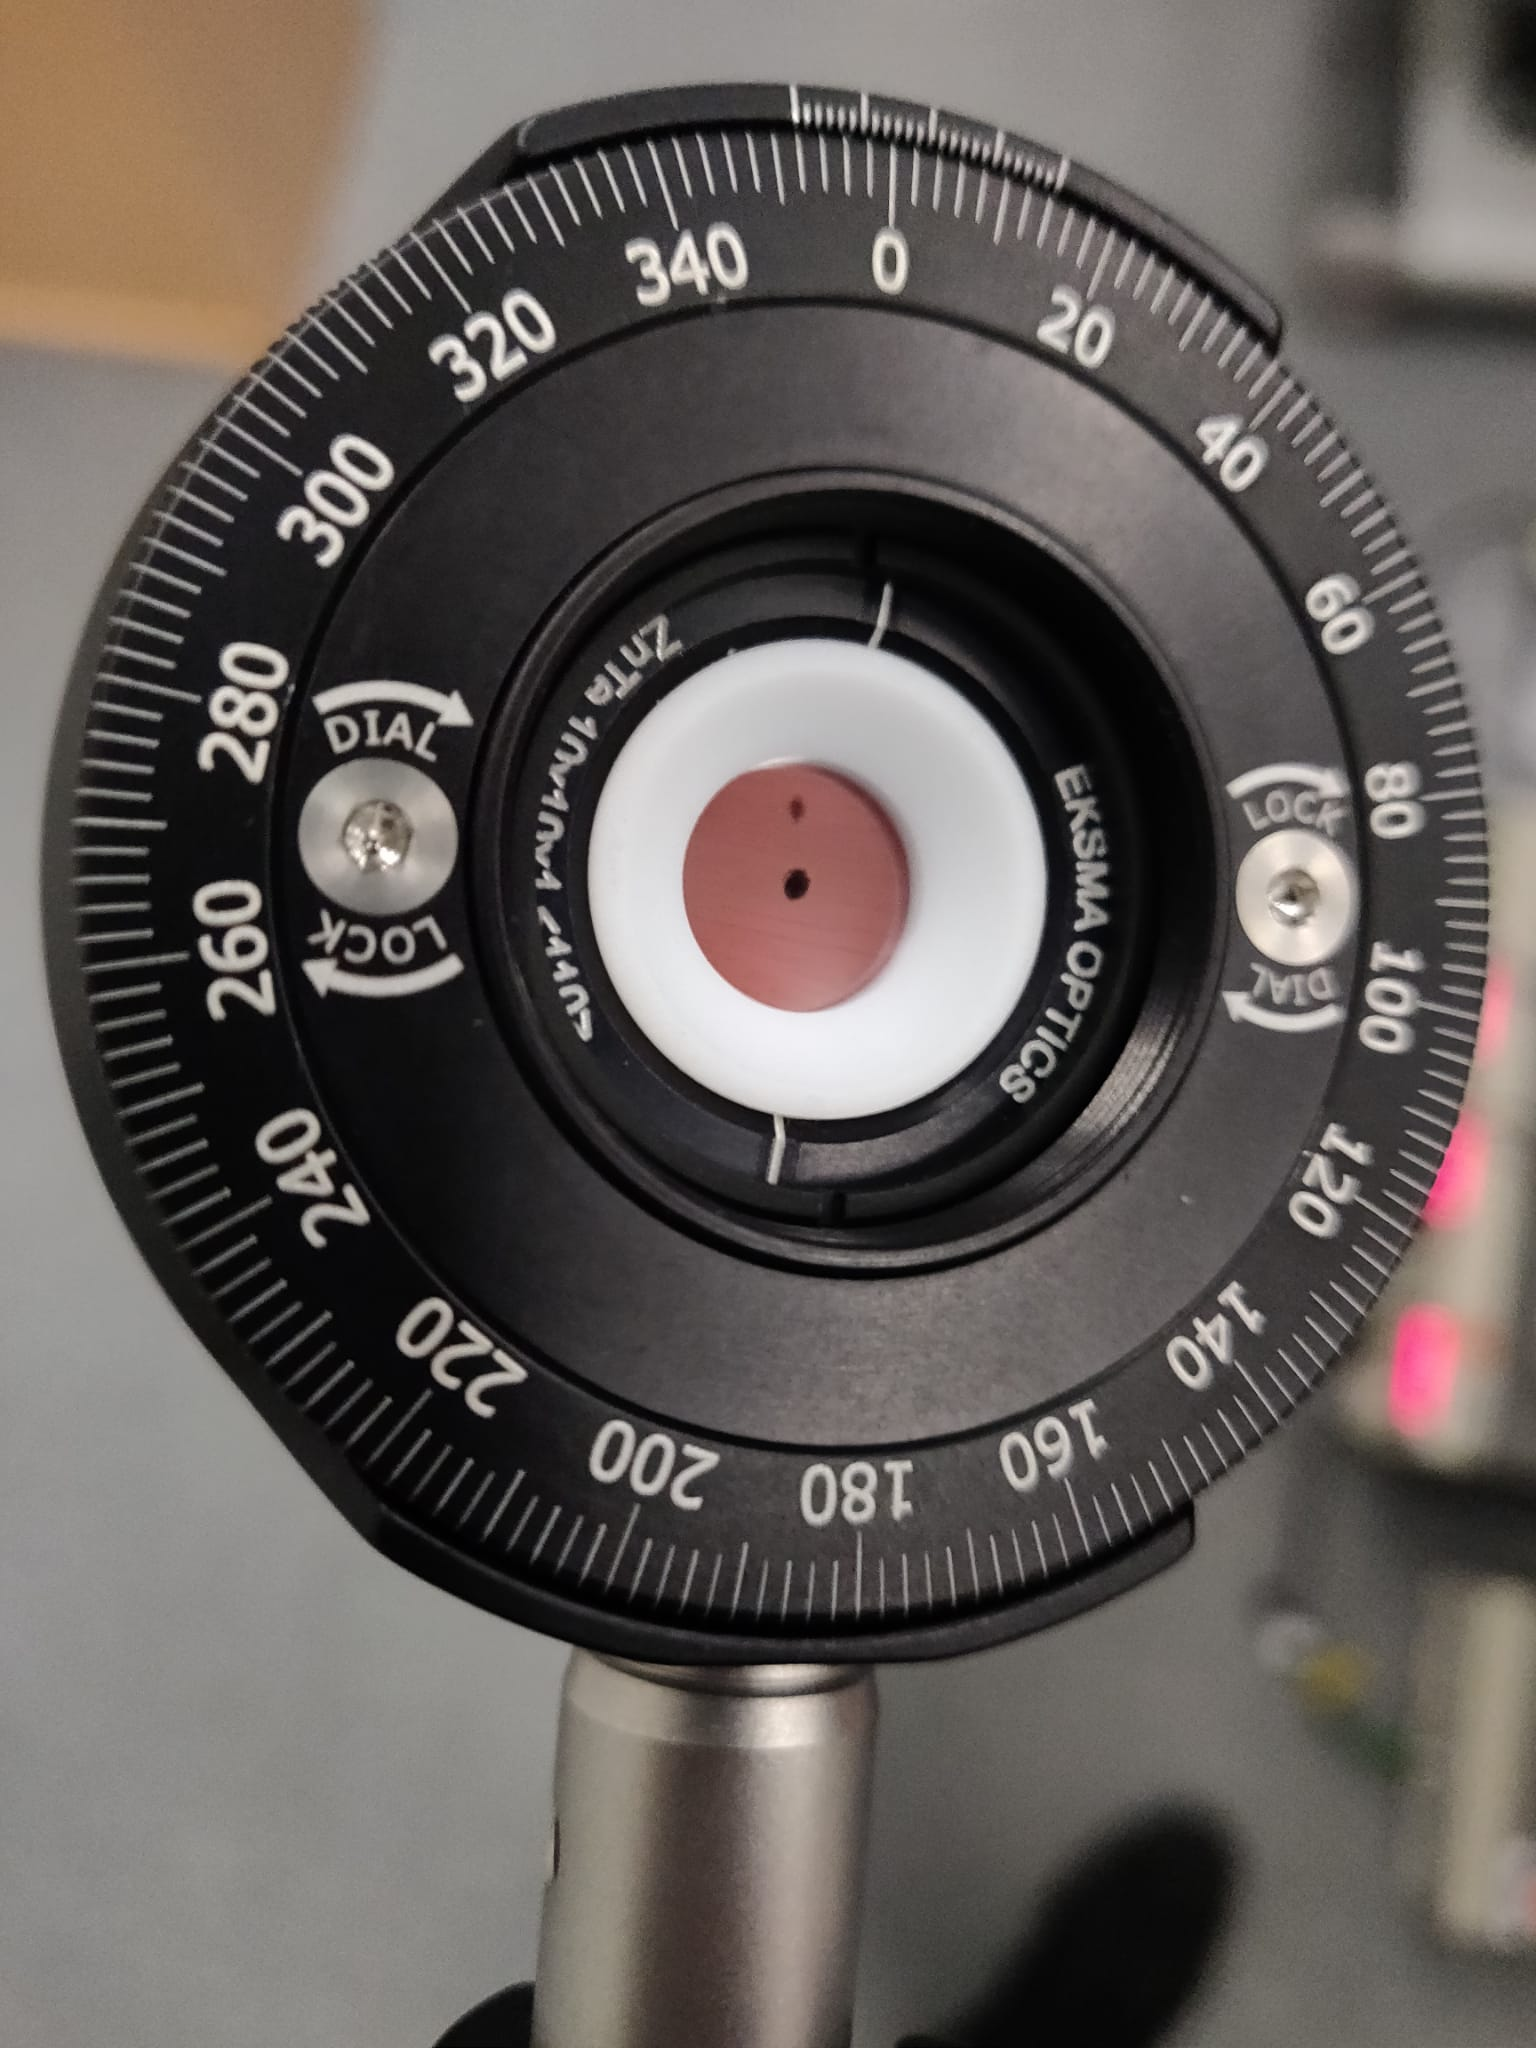
\includegraphics[width=0.5\textwidth]{Plots/burned_crystal.jpeg}
    \caption{The $\SI{1}{\milli\meter}$ ZnTe crystal that is used as the emitter.
    Two burned spots can cleary be seen on the crystal surface.}
    \label{fig:ZnTe_burned}
\end{figure}

\begin{figure}
    \centering
    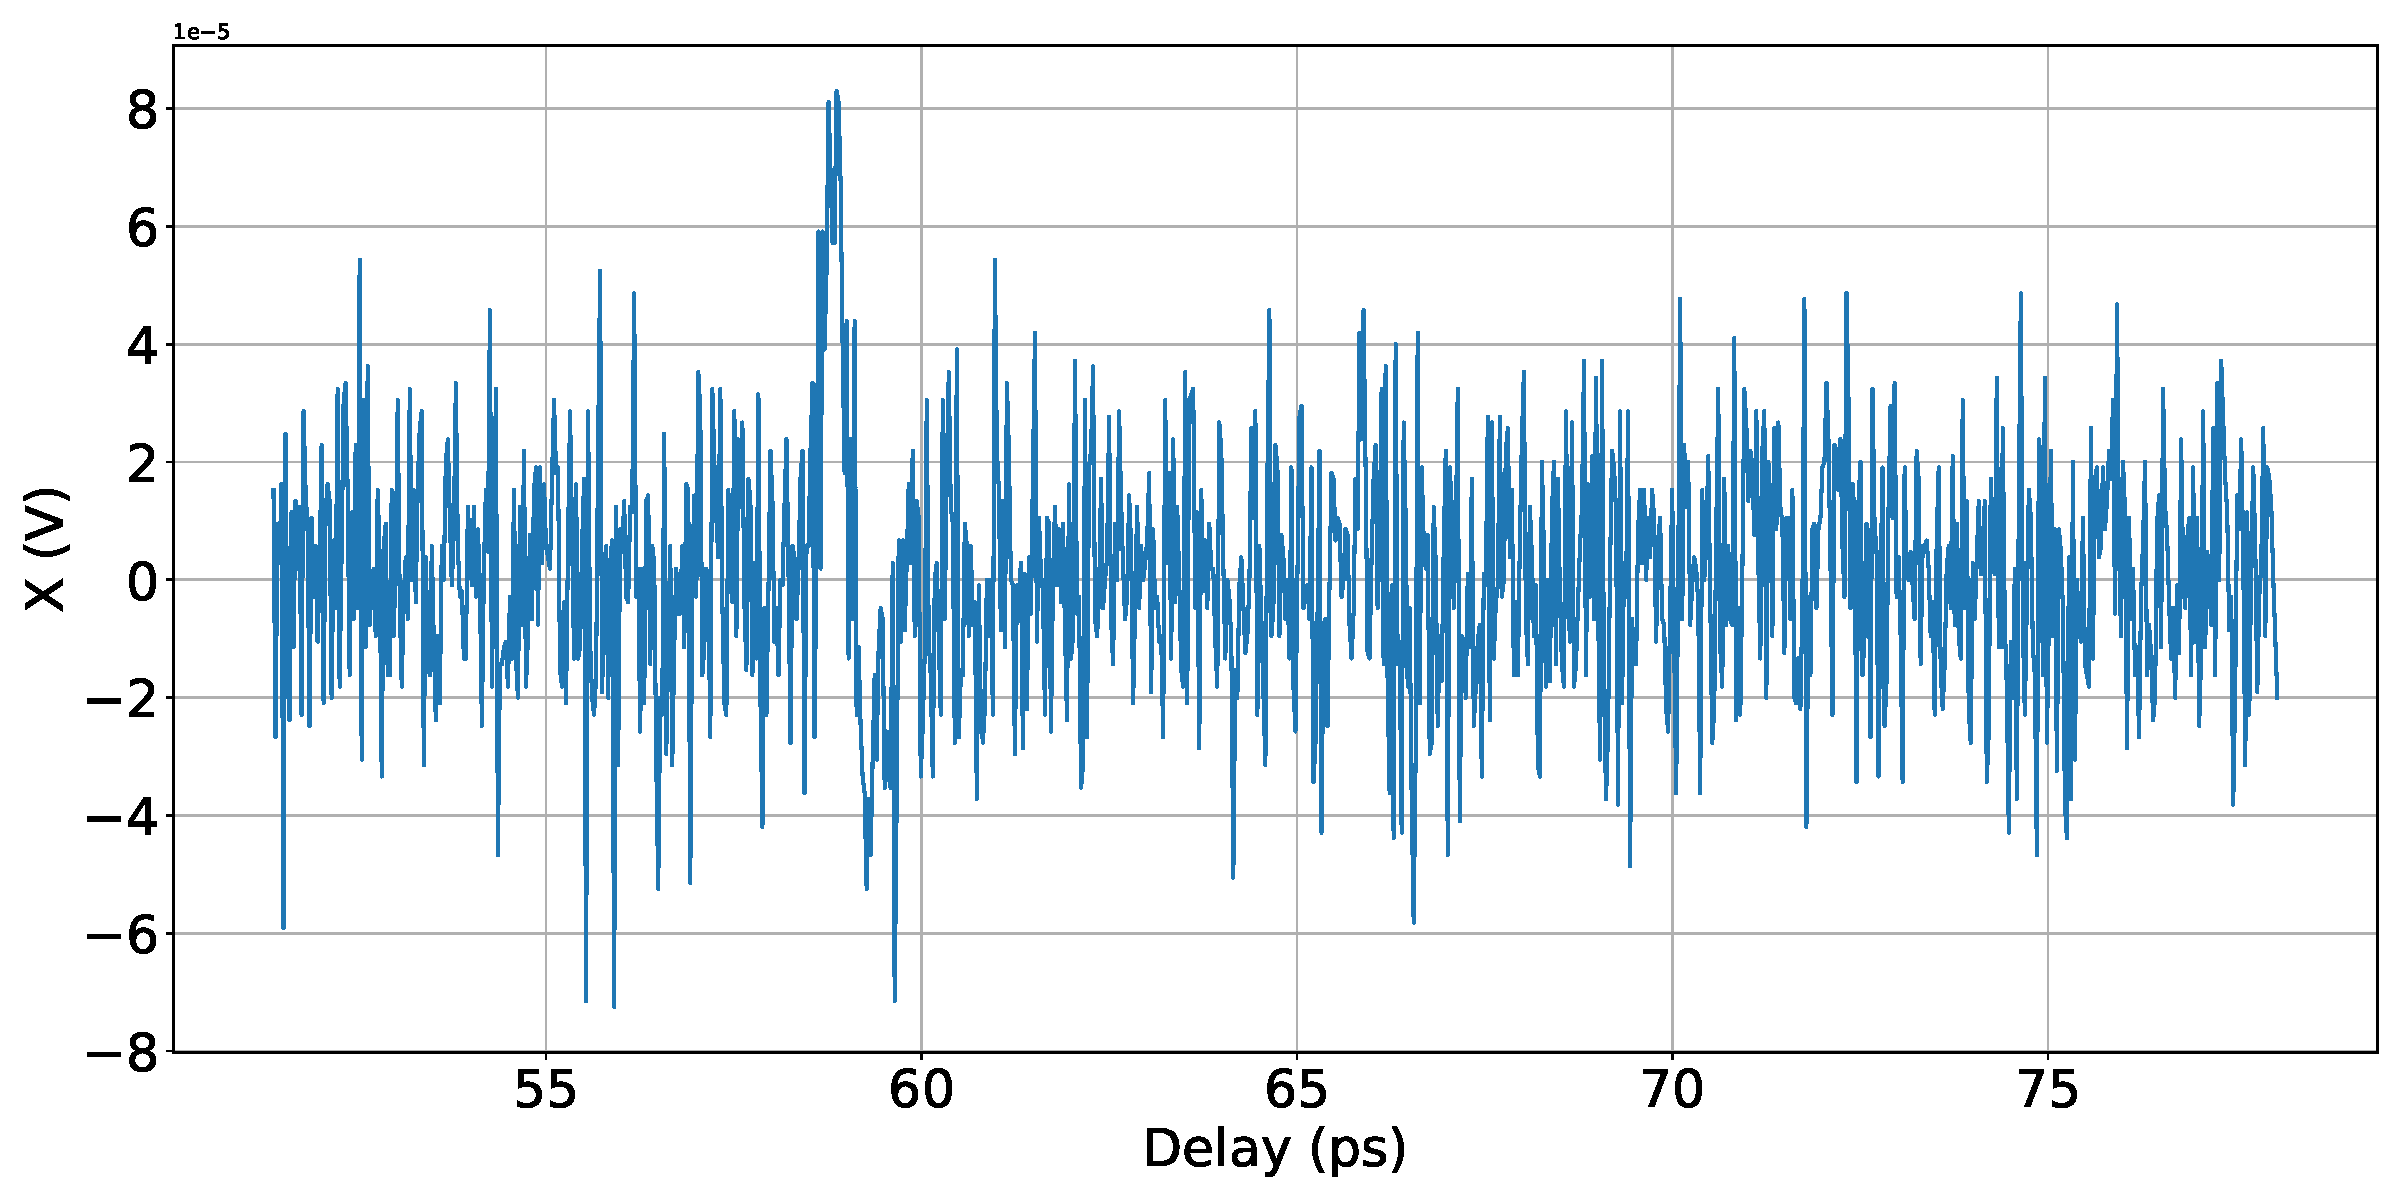
\includegraphics[width=0.5\textwidth]{Plots/GaP14_20_20normalX.pdf}
    \caption{A EOS signal with GaP as emitter crystal. A pump power of $\SI{24.2}{\milli\W}$ is used.
    The low pump power, combined with the thin crystal results in a very noisy measurement.}
    \label{fig:GaP_noise}
\end{figure}
